\begin{picture}(0,0)%
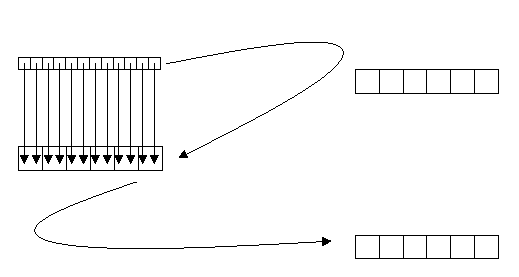
\includegraphics{figs/halving_operation.fig.eps}%
\end{picture}%
\setlength{\unitlength}{4144sp}%
%
\begingroup\makeatletter\ifx\SetFigFontNFSS\undefined%
\gdef\SetFigFontNFSS#1#2#3#4#5{%
  \reset@font\fontsize{#1}{#2pt}%
  \fontfamily{#3}\fontseries{#4}\fontshape{#5}%
  \selectfont}%
\fi\endgroup%
\begin{picture}(3686,1845)(256,-1288)
\put(271,434){\makebox(0,0)[lb]{\smash{{\SetFigFontNFSS{10}{12.0}{\familydefault}{\mddefault}{\updefault}{\color[rgb]{0,0,0}$r.row = n$}%
}}}}
\put(271,299){\makebox(0,0)[lb]{\smash{{\SetFigFontNFSS{10}{12.0}{\familydefault}{\mddefault}{\updefault}{\color[rgb]{0,0,0}$r.name = C$}%
}}}}
\put(2791,-916){\makebox(0,0)[lb]{\smash{{\SetFigFontNFSS{10}{12.0}{\familydefault}{\mddefault}{\updefault}{\color[rgb]{0,0,0}$out.row = n$}%
}}}}
\put(2791,-1051){\makebox(0,0)[lb]{\smash{{\SetFigFontNFSS{10}{12.0}{\familydefault}{\mddefault}{\updefault}{\color[rgb]{0,0,0}$out.name = C_{/2}$}%
}}}}
\put(2476,-196){\makebox(0,0)[lb]{\smash{{\SetFigFontNFSS{10}{12.0}{\familydefault}{\mddefault}{\updefault}{\color[rgb]{0,0,0}$out=new Row(C_{/2},n,\frac{p}{2})$}%
}}}}
\put(1441,-196){\makebox(0,0)[lb]{\smash{{\SetFigFontNFSS{10}{12.0}{\familydefault}{\mddefault}{\updefault}{\color[rgb]{0,0,0}$\sum_{/2}$}%
}}}}
\put(1981,434){\makebox(0,0)[lb]{\smash{{\SetFigFontNFSS{10}{12.0}{\familydefault}{\mddefault}{\updefault}{\color[rgb]{0,0,0}if $n$ is even}%
}}}}
\put(1306,-1096){\makebox(0,0)[lb]{\smash{{\SetFigFontNFSS{10}{12.0}{\familydefault}{\mddefault}{\updefault}{\color[rgb]{0,0,0}if $n$ is odd}%
}}}}
\end{picture}%
